

The SolKz benchmark is similar to the SolCx benchmark: 
the viscosity is a function of the space coordinates too and is given by 
\[
\eta(y)=\exp(2By) \quad {\rm with} \quad B=13.8155
\]
It is not a discontinuous function but grows exponentially with the 
vertical coordinate so that its overall variation is again $10^6$. 
The forcing is again chosen by imposing a spatially variable density variation as follows:
\[
\rho(x,y)=\sin(2y) \cos(3\pi y)
\]
Free slip boundary conditions are imposed on all sides of the domain.
This benchmark too is presented in \cite{zhon96} and is studied in \cite{dumg11} and \cite{gemd13}.

\begin{center}
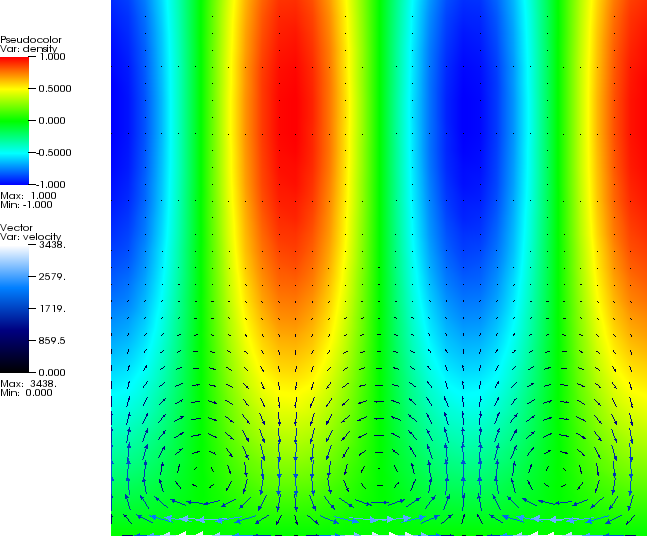
\includegraphics[width=6cm]{images/benchmark_solkz/solkz-solution}
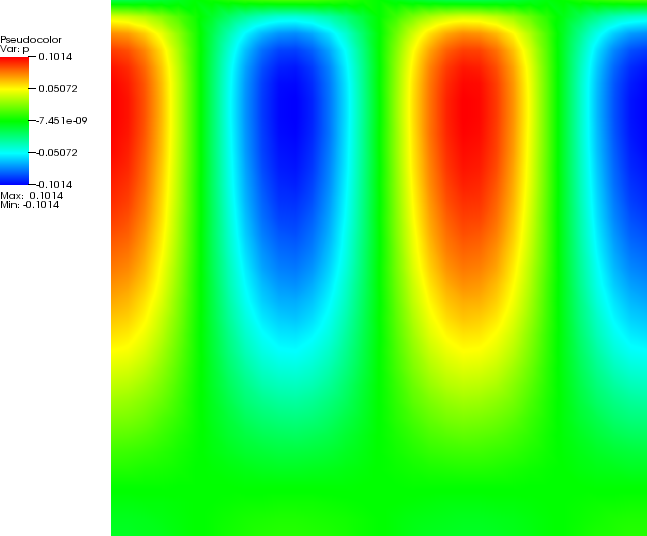
\includegraphics[width=6cm]{images/benchmark_solkz/solkz-solution-pressure}\\
{\captionfont Taken from \aspect manual \cite{aspectmanual}.}
\end{center}


\begin{center}
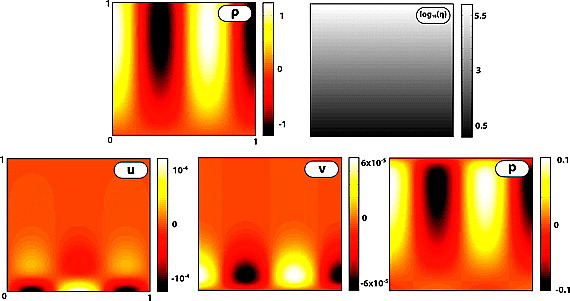
\includegraphics[width=10cm]{images/benchmark_solkz/dumg11}\\
{\captionfont Taken from Duretz \etal (2011) \cite{dumg11}.}
\end{center}

\Literature: \cite{mozg96}, \cite{mamo08}, \cite{vemmXX}, \cite{demh19}, \cite{repa87}
\stone 06
